\documentclass[12pt]{amsart}

%%%%%%%%%This project was adapted from Adam Graham-Squire at High Point University.

\addtolength{\hoffset}{-2.25cm}
\addtolength{\textwidth}{4.5cm}
\addtolength{\voffset}{-2.5cm}
\addtolength{\textheight}{5cm}
\setlength{\parskip}{0pt}
\setlength{\parindent}{0in}

\usepackage{amsthm, amsmath, amssymb, mathtools}
\usepackage[colorlinks = true, linkcolor = black, citecolor = black, final]{hyperref}
\usepackage{graphicx, multicol}
\usepackage{marvosym, wasysym}
\usepackage{tikz}
\usepackage{braket}
\usetikzlibrary{decorations.pathmorphing, shapes.geometric}

\usepackage{listings}
\usepackage{xcolor}

\definecolor{codegreen}{rgb}{0,0.6,0}
\definecolor{codegray}{rgb}{0.5,0.5,0.5}
\definecolor{codepurple}{rgb}{0.58,0,0.82}
\definecolor{backcolour}{rgb}{0.95,0.95,0.92}

\lstdefinestyle{mystyle}{
  backgroundcolor=\color{backcolour},   
  commentstyle=\color{codegreen},
  keywordstyle=\color{magenta},
  numberstyle=\tiny\color{codegray},
  stringstyle=\color{codepurple},
  basicstyle=\ttfamily\footnotesize,
  breakatwhitespace=false,         
  breaklines=true,                 
  captionpos=b,                    
  keepspaces=true,                 
  numbers=left,                    
  numbersep=5pt,                  
  showspaces=false,                
  showstringspaces=false,
  showtabs=false,                  
  tabsize=2
}

\lstset{style=mystyle}

\newcommand{\ds}{\displaystyle}
\DeclareMathOperator{\sech}{sech}



\pagestyle{empty}

\begin{document}

\thispagestyle{empty}

{\scshape FISI-4005} \hfill {\scshape \large Sergio Montoya Ramirez} \hfill {Tarea \#2\scshape }

\smallskip

\hrule

\section{}

Siguiendo las notas \textit{Eightfold way 16-04-2026-1.pdf}. Para las operaciones

\begin{align*}
  H_1 =
  \begin{pmatrix}
    1 &  0 & 0 \\
    0 & -1 & 0 \\
    0 &  0 & 0
  \end{pmatrix}; \quad
  H_2 =
  \begin{pmatrix}
    0 & 0 & 0 \\
    0 & 1 & 0 \\
    0 & 0 & -1
  \end{pmatrix}\\
  X_1 =
  \begin{pmatrix}
    0 & 1 & 0 \\
    0 & 0 & 0 \\
    0 & 0 & 0
  \end{pmatrix}; \quad
  X_2 =
  \begin{pmatrix}
    0 & 0 & 0 \\
    0 & 0 & 1 \\
    0 & 0 & 0
  \end{pmatrix}; \quad
  X_3 =
  \begin{pmatrix}
    0 & 0 & 1 \\
    0 & 0 & 0 \\
    0 & 0 & 0
  \end{pmatrix}\\
  Y_1 =
  \begin{pmatrix}
    0 & 0 & 0 \\
    1 & 0 & 0 \\
    0 & 0 & 0
  \end{pmatrix}; \quad
  Y_2 =
  \begin{pmatrix}
    0 & 0 & 0 \\
    0 & 0 & 0 \\
    0 & 1 & 0
  \end{pmatrix}; \quad
  Y_3 =
  \begin{pmatrix}
    0 & 0 & 0 \\
    0 & 0 & 0 \\
    1 & 0 & 0
  \end{pmatrix}\\
\end{align*}

Con la base:
\begin{align*}
  e_1 =
  \begin{pmatrix}
    1 \\ 0 \\ 0
  \end{pmatrix}; \quad
  e_2 =
  \begin{pmatrix}
    0 \\ 1 \\ 0
  \end{pmatrix}; \quad
  e_3 =
  \begin{pmatrix}
    0 \\ 0 \\ 1
  \end{pmatrix}
\end{align*}

\begin{itemize}
  \item Para el vector $\ket{e_1}$
    \begin{align*}
      H_1 \ket{e_1} &=
      \begin{pmatrix}
        1 &  0 & 0 \\
        0 & -1 & 0 \\
        0 &  0 & 0
      \end{pmatrix} 
      \begin{pmatrix}
        1 \\ 0 \\ 0
      \end{pmatrix}\\
      &= \begin{pmatrix}
        1 \\ 0 \\ 0
      \end{pmatrix} = \ket{e_1}\\
      H_2 \ket{e_1} &=
      \begin{pmatrix}
        0 &  0 & 0 \\
        0 &  1 & 0 \\
        0 &  0 & -1
      \end{pmatrix} 
      \begin{pmatrix}
        1 \\ 0 \\ 0
      \end{pmatrix}\\
      &= \begin{pmatrix}
        0 \\ 0 \\ 0
      \end{pmatrix} = 0\ket{e_1}\\
    \end{align*}

    Lo que implica que es un vector de peso con peso $(1, 0)$

  \item Para el vector $\ket{e_2}$
    \begin{align*}
      H_1 \ket{e_2} &=
      \begin{pmatrix}
        1 &  0 & 0 \\
        0 & -1 & 0 \\
        0 &  0 & 0
      \end{pmatrix} 
      \begin{pmatrix}
        0 \\ 1 \\ 0
      \end{pmatrix}\\
      &= \begin{pmatrix}
        0 \\ -1 \\ 0
      \end{pmatrix} = -1 \ket{e_2}\\
      H_2 \ket{e_2} &=
      \begin{pmatrix}
        0 &  0 & 0 \\
        0 &  1 & 0 \\
        0 &  0 & -1
      \end{pmatrix} 
      \begin{pmatrix}
        0 \\ 1 \\ 0
      \end{pmatrix}\\
      &= \begin{pmatrix}
        0 \\ 1 \\ 0
      \end{pmatrix} = \ket{e_2}\\
    \end{align*}

    Lo que implica que es un vector de peso con peso $(-1, 1)$

  \item Para el vector $\ket{e_3}$
    \begin{align*}
      H_1 \ket{e_3} &=
      \begin{pmatrix}
        1 &  0 & 0 \\
        0 & -1 & 0 \\
        0 &  0 & 0
      \end{pmatrix} 
      \begin{pmatrix}
        0 \\ 0 \\ 1
      \end{pmatrix}\\
      &= \begin{pmatrix}
        0 \\ 0 \\ 0
      \end{pmatrix} = 0 \ket{e_3}\\
      H_2 \ket{e_3} &=
      \begin{pmatrix}
        0 &  0 & 0 \\
        0 &  1 & 0 \\
        0 &  0 & -1
      \end{pmatrix} 
      \begin{pmatrix}
        0 \\ 0 \\ 1
      \end{pmatrix}\\
      &= \begin{pmatrix}
        0 \\ 0 \\ -1
      \end{pmatrix} = -1\ket{e_3}\\
    \end{align*}

    Lo que implica que es un vector de peso con peso $(0, -1)$
\end{itemize}

Ahora procesando todos los resultados con el código

\lstinputlisting[language=Python]{./codes/punto_1.py}

Obtenemos el resultado

\begin{align*}
  e_1 \otimes e_1 &= (2, 0)\\
  e_1 \otimes e_2 &= (0, 1)\\
  e_1 \otimes e_3 &= (1, -1)\\
  e_2 \otimes e_1 &= (0, 1)\\
  e_2 \otimes e_2 &= (-2, 2)\\
  e_2 \otimes e_3 &= (-1, 0)\\
  e_3 \otimes e_1 &= (1, -1)\\
  e_3 \otimes e_2 &= (-1, 0)\\
  e_3 \otimes e_3 &= (0, -2)\\
\end{align*}

Ahora agrupando los pesos simétricos en el anterior punto
\begin{align*}
  \psi_1 &= e_1 \otimes e_1 \text{ con peso } (2, 0)\\
  \psi_2 &= \frac{1}{\sqrt{2}} (e_1 \otimes e_2 + e_2 \otimes e_1) \text{ con peso } (0, 1)\\
  \psi_3 &= \frac{1}{\sqrt{2}} (e_1 \otimes e_3 + e_3 \otimes e_1) \text{ con peso } (1, -1)\\
  \psi_4 &= e_2 \otimes e_2 \text{ con peso } (-2, 2)\\
  \psi_5 &= \frac{1}{\sqrt{2}} (e_2 \otimes e_3 + e_3 \otimes e_2) \text{ con peso } (-1, 0)\\
  \psi_6 &= e_3 \otimes e_3 \text{ con peso } (0, -2)\\
\end{align*}

Y por el lado antisimétrico
\begin{align*}
  \phi_1 &= \frac{1}{\sqrt{2}} (e_1 \otimes e_2 - e_2 \otimes e_1) \text{ con peso } (0, 1)\\
  \phi_2 &= \frac{1}{\sqrt{2}} (e_1 \otimes e_3 - e_3 \otimes e_1) \text{ con peso } (1, -1)\\
  \phi_3 &= \frac{1}{\sqrt{2}} (e_2 \otimes e_3 - e_3 \otimes e_2) \text{ con peso } (-1, 0)\\
\end{align*}

Con lo cual ya encontramos los estados para $\mathbf{6}$ que descompone $3 \otimes 3 = \mathbf{6} \oplus \overline{\mathbf{3}}$.

\pagebreak

\section{}

Iniciando con
\begin{align*}
  dim(p, q) &= \frac{1}{2}(p + 1)(q + 1)(p + q + 2)\\
  dim(3, 0) &= \frac{1}{2}(3 + 1)(0 + 1)(3 + 0 + 2)\\
  &= \frac{1}{2}(4)(5)\\
  &= 10
\end{align*}

Ahora viendo las notas \textit{Clase-17} encontramos que las raices positivas simples son
\begin{itemize}
  \item $\alpha_1 = (2, -1)$
  \item $\alpha_2 = (-1, 2)$
\end{itemize}

Que se muestra en el documento \textit{El camino óctuple, parte 1-2.pdf} que todos los otros pesos son combinaciones lineales de esto. Ahora ademas tomando
\begin{align*}
  I_3 &= \frac{m_1}{2}\\
  Y &= \frac{1}{3}m_1 + \frac{2}{3}m_2
\end{align*}

Podemos desarrollar el siguiente codigo

\lstinputlisting[language=Python]{./codes/punto_2.py}

\begin{table}[h]
  \centering
  \renewcommand{\arraystretch}{1.5}
  \begin{tabular}{|c|c|c|c|c|c|}
    \hline
    \textbf{Particula} & \textbf{Peso $(m_1, m_2)$} & \textbf{$I_3$} & \textbf{$Y$} & \textbf{$S$} & \textbf{$Q$} \\ \hline
    $\Delta^{++}$ & $(3, 0)$ & $\frac{3}{2}$ & $1$ & $0$ & $2$ \\
    \hline
    $\Delta^{+}$ & $(1, 1)$ & $\frac{1}{2}$ & $1$ & $0$ & $1$ \\
    \hline
    $\Delta^{0}$ & $(-1, 2)$ & $\frac{-1}{2}$ & $1$ & $0$ & $0$ \\
    \hline
    $\Delta^{-}$ & $(-3, 3)$ & $\frac{-3}{2}$ & $1$ & $0$ & $-1$ \\
    \hline
    $\Sigma^{*+}$ & $(2, -1)$ & $1$ & $0$ & $-1$ & $1$ \\
    \hline
    $\Sigma^{*0}$ & $(0, 0)$ & $0$ & $0$ & $-1$ & $0$ \\
    \hline
    $\Sigma^{*-}$ & $(-2, 1)$ & $-1$ & $0$ & $-1$ & $-1$ \\
    \hline
    $\Xi^{*0}$ & $(1, -2)$ & $\frac{1}{2}$ & $-1$ & $-2$ & $0$ \\
    \hline
    $\Xi^{*-}$ & $(-1, -1)$ & $\frac{-1}{2}$ & $-1$ & $-2$ & $-1$ \\
    \hline
    $\Omega^{-}$ & $(0, -3)$ & $0$ & $-2$ & $-3$ & $-1$ \\
    \hline
  \end{tabular}
  \caption{Pesos del decuplete $\mathbf{10}$ con sus respectivos numeros cuanticos.}
  \label{tab:pesos_decuplete}
\end{table}

Con esto entonces obtenemos la figura
\begin{center}
  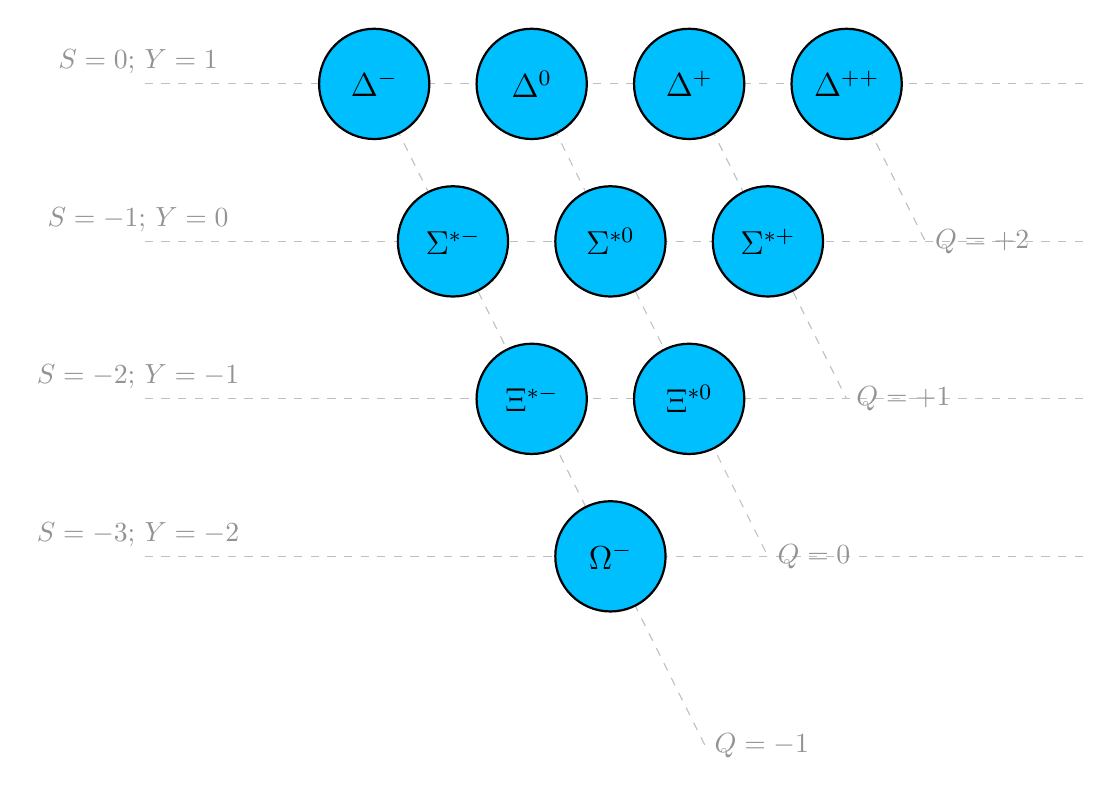
\begin{tikzpicture}[
      particle/.style = {
        circle, draw=black, fill=blue!25!cyan, thick, 
        minimum size=1.4cm, inner sep=0pt, 
        font=\large\bfseries, text=black
      }
    ]

    \draw[draw=gray!50, dashed, thin] (6,2)  -- (-6,2)  node[left,  above, gray!85] {$S=0;\, Y=1$};
    \draw[draw=gray!50, dashed, thin] (6,0)  -- (-6,0)  node[left,  above, gray!85] {$S=-1;\, Y=0$};
    \draw[draw=gray!50, dashed, thin] (6,-2) -- (-6,-2) node[left,  above, gray!85] {$S=-2;\, Y=-1$};
    \draw[draw=gray!50, dashed, thin] (6,-4) -- (-6,-4) node[left,  above, gray!85] {$S=-3;\, Y=-2$};

    \draw[draw=gray!50, dashed, thin] (-3,2) -- (0,-4) -- ++(1.2,-2.4)
      node[right, gray!85] {$Q=-1$};
    \draw[draw=gray!50, dashed, thin] (-1,2) -- (1,-2) -- ++(1.0,-2.0)
      node[right, gray!85] {$Q=0$};
    \draw[draw=gray!50, dashed, thin] (1,2)  -- (2,0)  -- ++(1.0,-2.0)
      node[right, gray!85] {$Q=+1$};
    \draw[draw=gray!50, dashed, thin] (3,2)  -- (4,0)
      node[right, gray!85] {$Q=+2$};

    \node[particle] (Delta++)    at ( 3, 2) {$\Delta^{++}$};
    \node[particle] (Delta+)     at ( 1, 2) {$\Delta^{+}$};
    \node[particle] (Delta0)     at (-1, 2) {$\Delta^{0}$};
    \node[particle] (Delta-)     at (-3, 2) {$\Delta^{-}$};

    \node[particle] (SigmaSplus)  at ( 2, 0) {$\Sigma^{*+}$};
    \node[particle] (SigmaSzero)  at ( 0, 0) {$\Sigma^{*0}$};
    \node[particle] (SigmaSminus) at (-2, 0) {$\Sigma^{*-}$};

    \node[particle] (XiSzero)  at ( 1,-2) {$\Xi^{*0}$};
    \node[particle] (XiSminus) at (-1,-2) {$\Xi^{*-}$};

    \node[particle] (Omega) at (0,-4) {$\Omega^{-}$};

  \end{tikzpicture}
\end{center}

Que corresponde exactamente con lo que esperamos. De hecho, como puede ver en el siguiente punto nos muestran esencialmente esta misma grafica.

\pagebreak

\section{}

Lo que podemos hacer para aproximarnos a una respuesta y dado que solamente tenemos dos pasos es mirar cual es la diferencia entre el primer y segundo paso y entre el segundo y el tercero.

\begin{align*}
  \Delta_{12} &= 1385 - 1232 = 153\\
  \Delta_{23} &= 1530 - 1385 = 145
\end{align*}

El promedio entre estos valores (que vamos a asumir es la diferencia para este siguiente paso) es $\Delta_{34} = \frac{153 + 145}{2} = 149$ y por tanto, esperariamos que el valor de la masa de la particula estuviese alrededor de
\begin{align*}
  m_{\Omega^{-}} &= 1530 + \Delta_{34}\\
  &= 1530 + 149\\
  &= 1679
\end{align*}

\end{document}
